\documentclass{boi2014-pl}

\usepackage{enumitem}

\renewcommand{\DayNum}{2}
\renewcommand{\TaskCode}{portals}
\renewcommand{\TaskName}{Portale}
\renewcommand{\TaskVersion}{1.1}

\newcommand{\constant}[1]{{\tt #1}}

\begin{document}
    \begin{wrapfigure}[4]{r}{4cm}
        \vspace{-24pt}
		\includegraphics[width=4cm]{\TaskCode.jpeg}
	\end{wrapfigure}

    W labiryncie znajduje się ciasto, a Ty masz na nie ogromną ochotę.
    Masz mapę labiryntu, która jest prostokątną planszą złożoną z $R$ wierszy oraz $C$ kolumn.
    Każda z komórek mapy zawiera jeden z następujących znaków:
    \begin{description}[itemindent=1pt]
    	\item[\constant{\#}] (hasz) oznaczający ścianę,
        \item[\constant{.}] (kropka) oznaczający wolne pole,
        \item[\constant{S}] (wielka litera s) oznaczający wolne pole, w którym się aktualnie znajdujesz,
        \item[\constant{C}] (wielka litera c) oznaczający wolne pole, w którym znajduje się ciasto.
    \end{description}

    Możesz poruszać się jedynie po wolnych polach oraz przechodzić między dwoma wolnymi polami,
    jeśli na mapie sąsiadują ze sobą bokiem.
    Dodatkowo, prostokątny obszar labiryntu opisany na mapie jest otoczony z zewnątrz przez ściany.

    Aby dobrać się do ciasta szybciej, zaopatrzyłeś się w urządzenie do tworzenia portali firmy
    Przysłona Nauka\texttrademark{}.
    W dowolnym momencie może ono wystrzelić portal w jednym z czterech kierunków: \emph{góra}, \emph{lewo}, \emph{dół}, \emph{prawo}.
    Gdy portal jest wystrzelony w pewnym kierunku, będzie się w nim poruszał, dopóki nie natrafi na ścianę.
    Wtedy pojawi się na ścianie, w którą trafił, po tej stronie ściany, w którą uderzył.
    
    W dowolnym momencie mogą istnieć co najwyżej dwa portale.
    Jeśli zdecydujesz się użyć urządzenia, gdy w labiryncie są już rozmieszczone dwa portale, jeden z nich (wybrany przez Ciebie) zostanie zniszczony.
    Wystrzelenie portalu w kierunku strony ściany, na której znajduje się już inny portal, zastąpi go (po każdej ze stron ściany może znajdować się co najwyżej jeden portal).
    Zauważ, że na jednej ścianie mogą znajdować się dwa portale, ale na różnych jej stronach.

    Jeśli w labiryncie są umieszczone dwa portale, możesz użyć ich do teleportacji.
    Stojąc przy jednym z portali, możesz pójść w jego kierunku, w wyniku czego znajdziesz się na wolnym polu sąsiadującym z drugim portalem.
    Zajmuje to tyle samo czasu, co przejście między sąsiednimi polami.

    Możesz założyć, że wystrzelenie portalu nie zajmuje czasu, a przemieszczenie się między sąsiednimi polami labiryntu oraz teleportacja przy użyciu portali zajmuje jednostkę czasu.

    \Task
    Mając daną mapę labiryntu wraz z Twoją pozycją startową oraz pozycją ciasta, wyznacz najkrótszy czas, w jakim możesz dobrać się do smakołyku.

    \Input
    W pierwszym wierszu wejścia znajdują się dwie liczby całkowite: liczba wierszy mapy $R$ oraz liczba kolumn mapy $C$.
    Kolejne $R$ wierszy opisuje mapę.
    Każdy z nich zawiera $C$ znaków: \constant{\#}, \constant{.}, \constant{S} i/lub \constant{C} (których znaczenie wyjaśnione jest na górze).

    Każdy ze znaków \constant{S} oraz \constant{C} pojawi się na wejściu dokładnie raz.

    \Output
    Wyjście powinno zawierać jedną liczbę całkowitą -- najkrótszy czas, w jakim możesz dostać się do ciasta z Twojej pozycji startowej.

    Możesz założyć, że droga do ciasta zawsze istnieje.

    \Example
    \example
    {
        4 4\newline
        .\#.C\newline
        .\#.\#\newline
        ....\newline
        S...
    }
    {
        4
    }
    {
        Jeden z najkrótszych sposobów dojścia do ciasta to: 1) zrób krok w prawo, 2) zrób krok w prawo, wystrzel jeden portal do góry i jeden w dół, 3) przejdź przez dolny portal, 4) zrób krok w prawo i zjedz ciasto.

        \begin{center}
            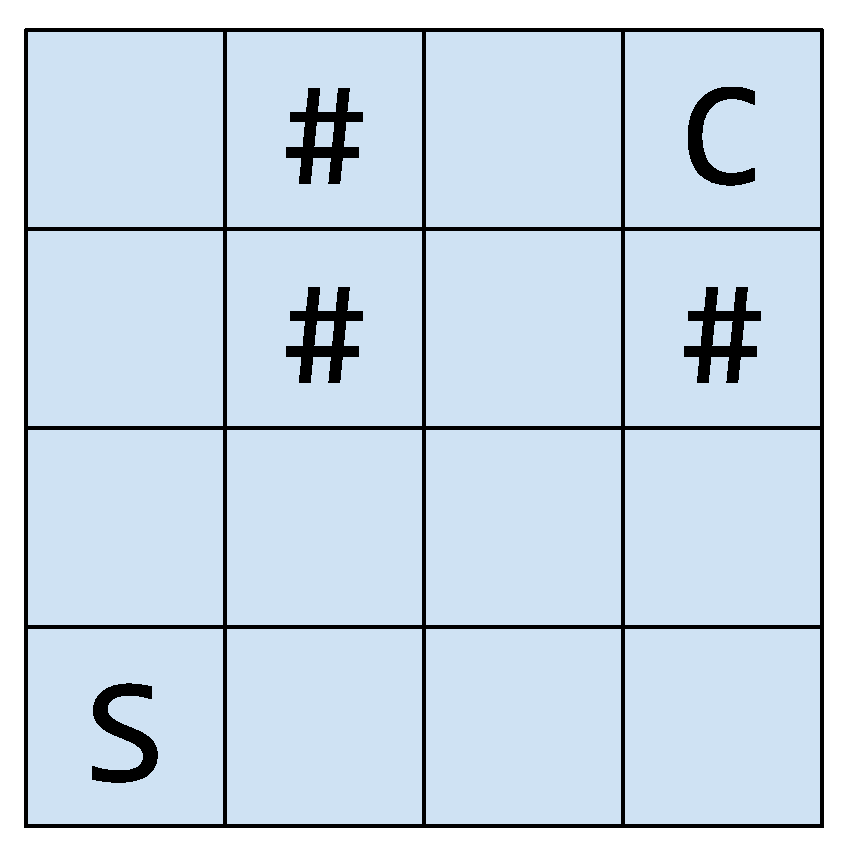
\includegraphics[width=4cm]{portals-example}
        \end{center}
    }

    \Scoring

    \begin{description}[leftmargin=0pt]
        \item[Podzadanie 1 (11 punktów):] $1 \le R \le 10, 1 \le C \le 10$.
        \item[Podzadanie 2 (20 punktów):] $1 \le R \le 50, 1 \le C \le 50$.
        \item[Podzadanie 3 (20 punktów):] $1 \le R \le 200, 1 \le C \le 200$.
        Każde wolne pole ma co najmniej jedną sąsiadującą z nim ścianę.
        \item[Podzadanie 4 (19 punktów):] $1 \le R \le 200, 1 \le C \le 200$.
        \item[Podzadanie 5 (30 punktów):] $1 \le R \le 1\,000, 1 \le C \le 1\,000$.
    \end{description}

    \Constraints

    \begin{description}
        \item[Limit czasu:] 1 s.
        \item[Dostępna pamięć:] 256 MB.
    \end{description}
\end{document}
